\section{Pronunciation Reconstruction Model} \label{sec:model}
In this section, we introduce the architecture of our pronunciation reconstruction model, centered around \figref{fig:model_structure}. By utilizing an embedding layer and a transformer encoder layer, our model is capable of learning complex patterns and relationships within both the phonetic data and the glyph information, enabling accurate reconstructions across different historical periods.

\subsection{Model Architecture}
As shown in \figref{fig:model_structure}, our glyph and temporal enhanced (\textbf{GTenhanced}) pronunciation reconstruction model consists of an embedding layer and a transformer encoder layer.

\begin{figure*}
    \centering
    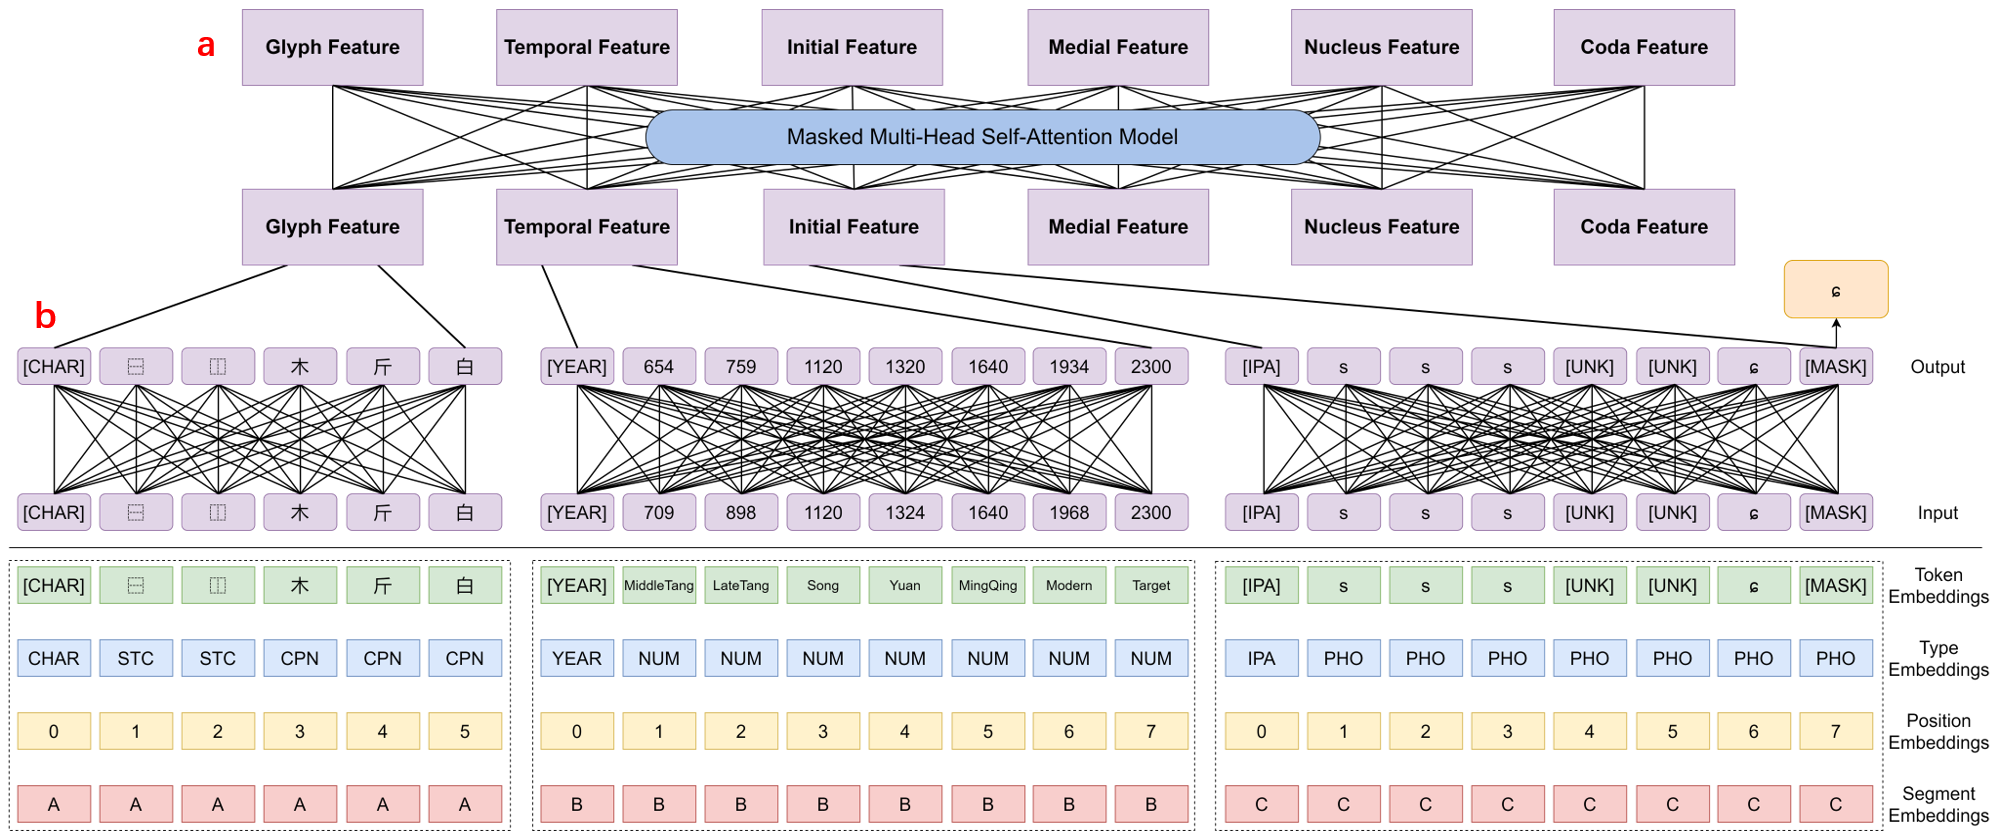
\includegraphics[width=1\textwidth]{images/embedding.png}
    \caption{\textbf{Architecture of glyph and temporal enhanced ancient Chinese pronunciation reconstruction model.} \textbf{(a)} Using a feature-differentiated block architecture, the model transmits attention between blocks through markers such as [CHAR], [YEAR], and [IPA]. \textbf{(b)} The embedding of glyph feature, temporal feature and initial feature. The embedding for medial feature, nucleus feature, and coda feature are constructed similarly to the embedding for initial feature. The detailed embedding can be found in \appref{app:embedding}.}
    \label{fig:model_structure}
\end{figure*}

First, for the feature representation of Chinese character glyph, we build upon the approach of \citet{lyu2021glyph}. Specifically, using the Han Ideographs structure files\footnote{\url{https://github.com/tomcumming/chise-ids}}, we follow the methodology outlined by \citet{ke2017radical}\footnote{\url{https://github.com/yuanzhiKe/Radical\_CR\_Encoder}} to generate glyph trees for all Chinese characters in our dataset. Each glyph tree is then converted into a sequence format using a depth-first algorithm, as described by \citet{nguyen2019hierarchical}. As shown in \figref{fig:glyph_embedding}, the input sequence comprises two distinct token types: leaf nodes (positions 3, 4, 5) representing components of Chinese characters, and internal nodes (positions 1, 2) representing structural operators (e.g., left-right). These token types will be utilized for glyph type embedding. The positions of these tokens (0, 1, 2, 3, 4, 5) denote the sequence order in the input and will subsequently be utilized for glyph position embedding, as shown in \figref{fig:model_structure}.

Next, for the feature representation of Chinese character pronunciations, we segments the syllable of a Chinese character into four parts, as mentioned in \secref{sec:dataset}. The entire input sequence consists of the character glyph sequence, the temporal sequence, and the sequences of phonetic changes over time for each part of the syllable. For example, the final sequence representation for the character \begin{CJK*}{UTF8}{gbsn}
“皙”
\end{CJK*} can be serialized as shown in \figref{fig:model_structure}.

\begin{figure}[ht]
    \centering
    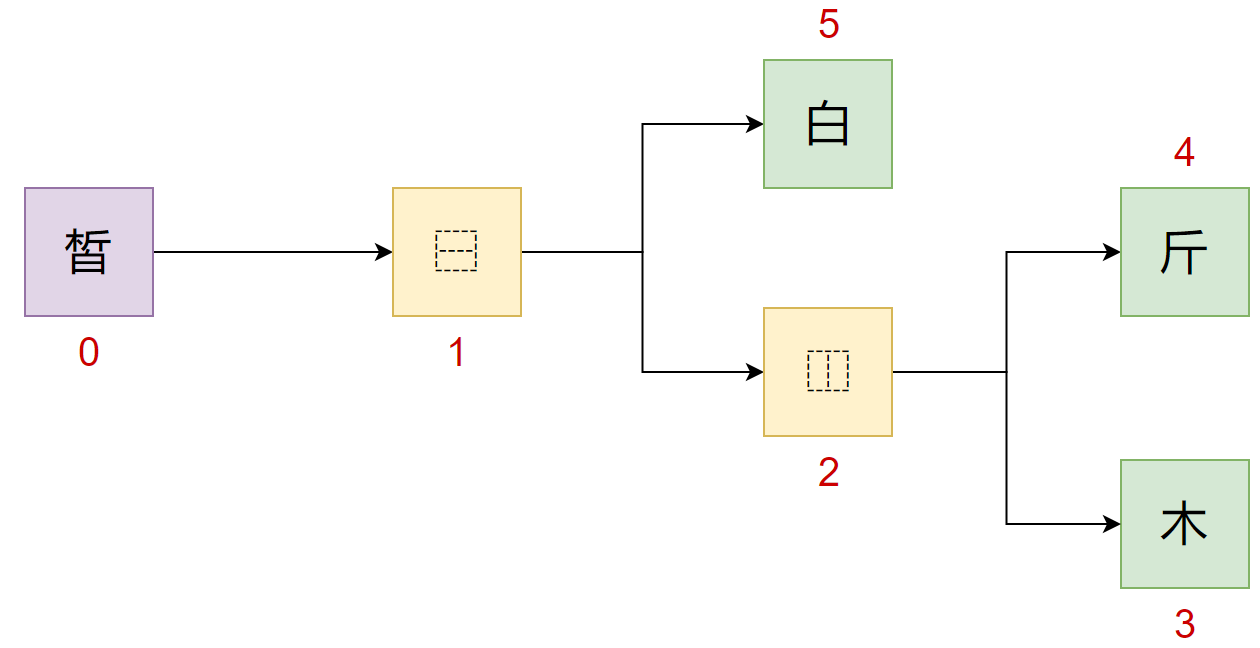
\includegraphics[width=0.4\textwidth]{images/character_tree.png}
    \caption{The glyph tree of a Chinese character. }
    \label{fig:glyph_embedding}
\end{figure}

\subsection{Embedding Layer}
The model input embedding is the combination of \texttt{token, type, position, and character segmentation} embeddings, as shown in \figref{fig:glyph_embedding}.
%\MY{use concatenation or combination, it's not sum}
%the embedding of these features is visually represented in \figref{fig:model_structure2}

\noindent\textbf{Token Embedding} encodes glyph, temporal and phoneme features in different segments started by token [CHAR], [YEAR] and [IPA] and followed by glyph, temporal and phoneme information. Additionally we use [MASK] to mask the phoneme tokens, use [UNK] to fill in the unknown Yuan and MingQing phoneme data.

\noindent\textbf{Type Embedding}  distinguishes token types: for glyph feature tokens, ``CHAR'' denotes the character tag [CHAR], ``STC'' and ``CPN'' represents the structure and component type; for temporal features, ``YEAR'' marks the period tag [YEAR] and ``NUM'' signifies the numerically encoded year information; for phoneme tokens, ``IPA'' labels the phoneme tag [IPA], while ``PHO'' designates the phoneme.

\noindent\textbf{Position Embedding} assigns a number starting from 0 to each token within the same feature, helping the model understand token positions in their respective sequences.

\noindent\textbf{Segmentation Embedding} identifies different features, helping the model distinguish between character glyph, historical periods, and phonetic changes. All the embedding have the same dimension $d$.

\subsection{Masked Transformer Encoder}
We utilize the multi-head self-attention network as the foundational structure. Given a sequence of tokens represented by $\mathbf{X} \in \mathbb{R}^{n \times d}$, where $n$ denotes the number of tokens in the sequence and $d$ represents the dimension of each token, the process of masked self-attention can be formulated as follows:

\begin{align*}
\mathbf{A} &=\frac{(\mathbf{X} \mathbf{W}^{Q})(\mathbf{X} \mathbf{W}^{K})^{\top}}{\sqrt{d_{k}}} \\
\widetilde{\mathbf{X}} &=\operatorname{Softmax}(\mathbf{A}+\mathbf{M})(\mathbf{X} \mathbf{W}^{V}),
\end{align*}
\noindent
where $\mathbf{W}^{Q}, \mathbf{W}^{K}, \mathbf{W}^{V} \in \mathbb{R}^{d \times d_{k}}$ serve as learnable parameters, while $\mathbf{M} \in \mathbb{R}^{n \times n}$ denotes the attention mask matrix~\cite{liu2020k}. We derive $\mathbf{M}$ by setting $\mathbf{M}_{ij}$ to 0 when $x_{j}$ is visible to $x_{i}$, and to $-\infty$ when $x_{j}$ is invisible to $x_{i}$. Specifically, all tokens within the same feature are mutually visible to each other; additionally, the special tags [CHAR], [YEAR], and [IPA] are also mutually visible to each other. The Softmax function is applied to the attention scores to normalize them into a probability distribution, ensuring that the weights sum to one.

\subsection{Training Target}
Inspired by the training methodology of BERT~\cite{devlin2018bert}, we randomly mask 15\% of the phoneme tokens in the input sequence. Within this 15\%, 80\% are replaced by the mask token [MASK], 10\% are randomly replaced by a token belonging to the same token type, and 10\% remain unchanged. Consequently, the model is trained to predict the original phoneme tokens based on the modified input, as illustrated in the top-right of \figref{fig:model_structure}(b).

% \begin{figure*}[ht]
%     \centering
%     \begin{subfigure}[b]{\textwidth}
%         \centering
%         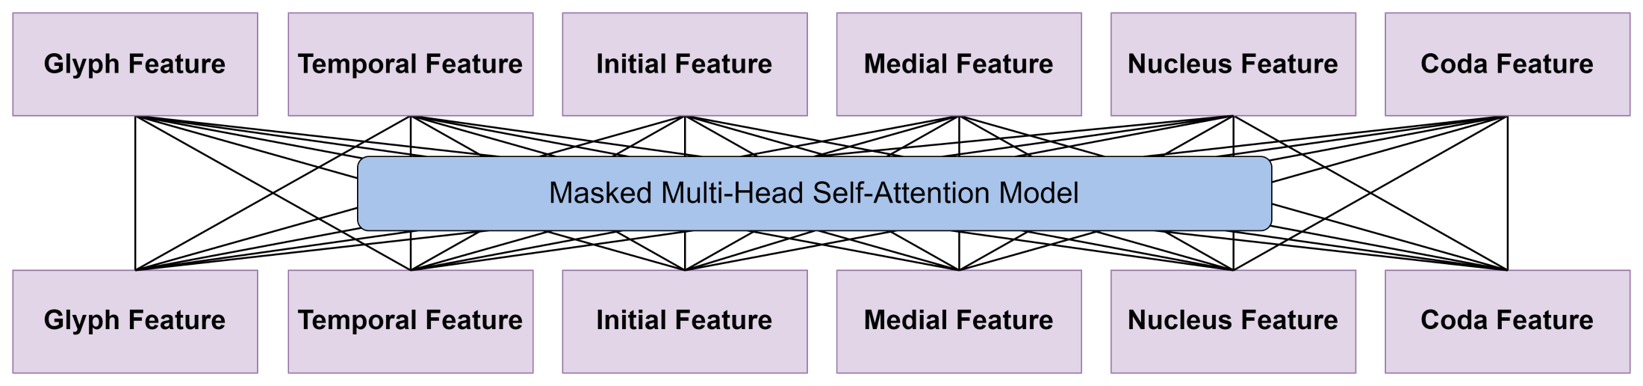
\includegraphics[width=0.9\textwidth]{images/overview_architecture.png}
%         \caption{Using a feature-differentiated block architecture, the model transmits attention between blocks through markers such as [CHAR], [YEAR], and [IPA].}
%         \label{fig:model_structure1}
%     \end{subfigure}
%     \vskip\baselineskip
%     \begin{subfigure}[b]{\textwidth}
%         \centering
%         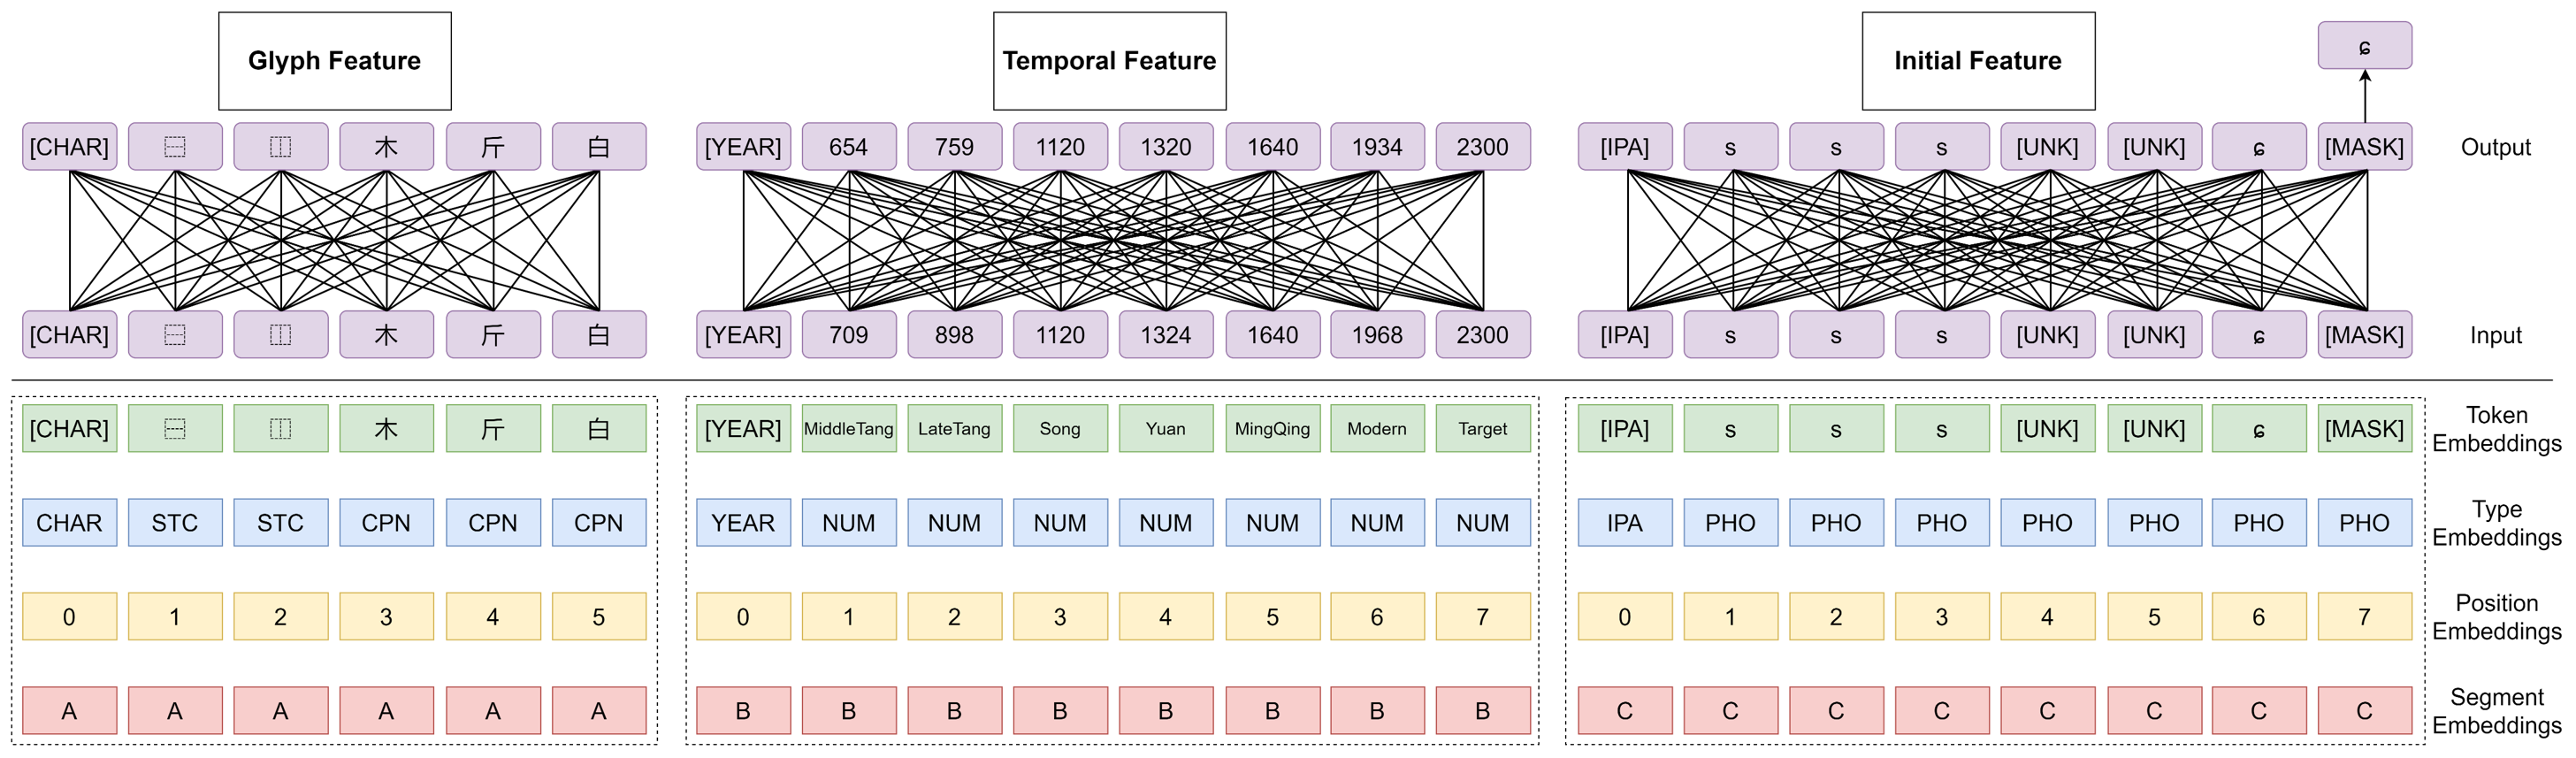
\includegraphics[width=1\textwidth]{images/embedding_layer1.png}
%         \caption{The embedding of glyph feature, temporal feature and initial feature. The embedding for medial feature, nucleus feature, and coda feature are constructed similarly to the embedding for initial feature. The detailed embedding can be found in \appref{app:embedding}.}
%         \label{fig:model_structure2}
%     \end{subfigure}
%     \caption{Architecture of glyph and temporal enhanced ancient Chinese pronunciation reconstruction model.}
%     \label{fig:model_structure}
% \end{figure*}